\documentclass[../solutions_manual.tex]{subfiles}
\begin{document}
\ifSubfilesClassLoaded{\setcounter{chapter}{11}}{}% NN-1 when built standalone
\setcounter{chapter}{11}% NN-1, so this chapter is numbered NN
\chapter{Welfare Under Endogenous Preferences}\label{sol12}
\sloppy

All numbers below are printed by \texttt{python3} \nolinkurl{code/solutions/sol12.py}. Throughout, $v(z) = z - \frac{\kappa}{2}z^2$ (equation~\eqref{ch12:eq:refdep}) and aspirations are $\mathbf{a} = \mathcal{M}W^I\x$ (equation~\eqref{ch12:eq:aspiration}). The stylized Bolivia allocation of Example~\ref{ch10:ex:bolivia_three} is $\bar x_b = (1.2486, 0.9852, 0.7662)$, with three agents per block.

%% ---------------------------------------------------------------------
\exercisesolution{12.1}{The satisfaction paradox}
\textbf{Computation} ($\kappa = 0.5$, the near-block-diagonal $W^I$ of Example~\ref{ch12:ex:satisfaction}; every $\kappa z < 1$):
\begin{center}
\small
\begin{tabular}{lccccc}
\toprule
$\mathcal{M}$ & $a_b$ (block $W^I$) & $s_b$ (block $W^I$) & gap & gap with $\Wce$ & ratio \\
\midrule
0   & $(0, 0, 0)$ & $(0.8588, 0.7425, 0.6194)$ & 0.2394 & 0.2394 & 1.000 \\
0.4 & $(0.4771, 0.3954, 0.3275)$ & $(0.6227, 0.5028, 0.3906)$ & 0.2321 & 0.3359 & 0.691 \\
0.8 & $(0.9541, 0.7908, 0.6550)$ & $(0.2728, 0.1849, 0.1081)$ & 0.1647 & 0.4324 & 0.381 \\
\bottomrule
\end{tabular}
\end{center}
The gas-minus-rural gap as a function of $\mathcal{M}$ (on a grid of $0.1$):
\begin{center}
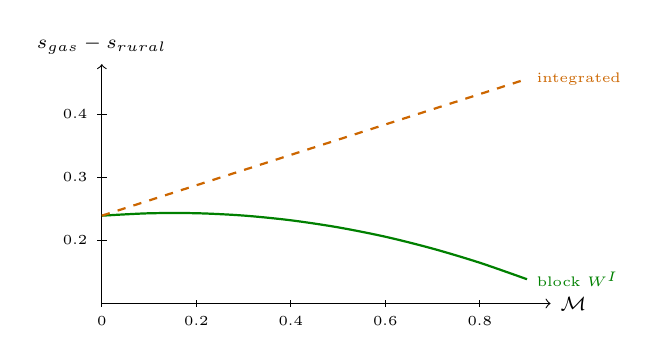
\begin{tikzpicture}[xscale=6, yscale=8]
\draw[->] (0,0.1) -- (0.95,0.1) node[right, font=\scriptsize] {$\mathcal{M}$};
\draw[->] (0,0.1) -- (0,0.48) node[above, font=\scriptsize] {$s_{\text{gas}} - s_{\text{rural}}$};
\foreach \m in {0,0.2,0.4,0.6,0.8} {\draw (\m,0.105) -- (\m,0.095) node[below, font=\tiny] {\m};}
\foreach \y in {0.2,0.3,0.4} {\draw (0.01,\y) -- (-0.01,\y) node[left, font=\tiny] {\y};}
\draw[thick, green!50!black] plot[smooth] coordinates {(0.0,0.2394) (0.1,0.2432) (0.2,0.2433) (0.3,0.2396) (0.4,0.2321) (0.5,0.2209) (0.6,0.2060) (0.7,0.1872) (0.8,0.1647) (0.9,0.1385)};
\draw[thick, orange!80!black, dashed] plot coordinates {(0.0,0.2394) (0.9,0.4565)};
\node[font=\tiny, green!50!black, right] at (0.9,0.1385) {block $W^I$};
\node[font=\tiny, orange!80!black, right] at (0.9,0.4565) {integrated $\Wce$};
\end{tikzpicture}
\end{center}
With integrated aspirations, everyone has the same aspiration $\mathcal{M}\bar x$. The gap is then $(x_1 - x_3)[1 - \kappa((x_1 + x_3)/2 - \mathcal{M}\bar x)]$, which is linear and increasing in $\mathcal{M}$, from $0.2394$ to $0.4565$ at $\mathcal{M} = 0.9$. With the near-block $W^I$, the gap is a concave quadratic in $\mathcal{M}$ (constant second differences $-0.0038$). It rises slightly up to $\mathcal{M} \approx 0.15$ and then falls, to $0.1647$ at $\mathcal{M} = 0.8$. The slight initial rise comes from the cross-block weights ($0.025$): each block's aspiration includes a little of the others' allocations, and the concavity of $v$ interacts with it. For large $\mathcal{M}$ the compression dominates. The ratio to the integrated gap ($0.381$ at $\mathcal{M} = 0.8$) is above $1 - \mathcal{M} = 0.2$, because $W^I$ is not exactly block-diagonal and there are three blocks.

\textbf{Verification of Proposition~\ref{ch12:thm:paradox}} (two equal blocks, pure block-diagonal $W^I$). We give a route different from the book's. For quadratic $v$, the midpoint rule is exact:
\[
v(z_1) - v(z_2) = \int_{z_2}^{z_1}(1 - \kappa z)\,dz = (z_1 - z_2)\,v'\!\Big(\frac{z_1 + z_2}{2}\Big).
\]
\begin{itemize}
\item \emph{Block-diagonal:} $z_b = x_b - \mathcal{M}x_b = (1-\mathcal{M})x_b$. So $z_M - z_T = (1-\mathcal{M})(x_M - x_T)$, with midpoint $(1-\mathcal{M})\bar x$, where $\bar x = (x_M + x_T)/2$.
\item \emph{Integrated:} $z_b = x_b - \mathcal{M}\bar x$. So $z_M - z_T = x_M - x_T$, with midpoint $\bar x - \mathcal{M}\bar x = (1-\mathcal{M})\bar x$.
\end{itemize}
The midpoints coincide, so the $v'$ factors are equal. They are positive because every $\kappa z < 1$ implies $\kappa\cdot$midpoint $< 1$. Hence the ratio of the gaps is $(1-\mathcal{M})(x_M - x_T)/(x_M - x_T) = 1 - \mathcal{M}$. $\square$ Numerically, at $(x_M, x_T) = (1.2, 0.8)$ and $\kappa = 0.5$: for $\mathcal{M} = 0.4$ the gaps are $0.168$ and $0.280$ (ratio $0.600$); for $\mathcal{M} = 0.8$ they are $0.072$ and $0.360$ (ratio $0.200$). The exactness is special to quadratic $v$. With $v(z) = \ln(1+z)$ and $\mathcal{M} = 0.8$, the ratio is $0.198$ instead of $0.2$.

%% ---------------------------------------------------------------------
\exercisesolution{12.2}{Laundered aspirations}
With $W^I_{\text{just}} = \frac19\ones\ones' = \Wce$ and $\x^{\text{ref}}$ the current allocation, Proposition~\ref{ch12:prop:laundered}(1) gives a common laundered aspiration $\hat a = \mathcal{M}\bar x = 0.8\times 1.0000 = 0.8$ ($\mathcal{M} = 0.8$, $\kappa = 0.5$). Laundered satisfaction by block is
\[
v(\bar x_b - 0.8) = (0.3983,\ 0.1766,\ -0.0341).
\]
The \emph{rural} block has negative laundered satisfaction: its allocation $0.766$ is below the aspiration $0.8$ it would hold if it observed the whole economy.

\textbf{Ranking the current allocation against $\bar x_b = 1$}, with $W_1 = \sum_i v(x_i - a_i^*(\x))$ and $W_2 = \sum_i v(x_i - 0.8)$:
\begin{center}
\begin{tabular}{lcc}
\toprule
& endogenous $W_1$ & laundered $W_2$ \\
\midrule
current $\x$ & 1.6974 & 1.6225 \\
equal $\x = \ones$ & 1.7100 & 1.7100 \\
difference (equal $-$ current) & 0.0126 & 0.0875 \\
\bottomrule
\end{tabular}
\end{center}
The ranking does \emph{not} change: both criteria prefer the equal allocation. The size of the gain does change. The endogenous criterion records a gain seven times smaller ($0.0126$ vs.\ $0.0875$), because under $W^I$ the rural block's aspirations are low (0.655), so the rural shortfall that equalization cures is mostly invisible to it. The ranking survives here for a structural reason. This $W^I$ is symmetric, hence doubly stochastic (all column sums equal 1). By Proposition~\ref{ch12:prop:endo_linear}, the linear part of $W_1$ is then $(1-\mathcal{M})\Omega = 1.8$ for \emph{every} allocation. Only the concave part differs, and that part always favours equality. With a $W^I$ that is not doubly stochastic, the endogenous criterion depends on who is watched. With the ``media hub'' of Chapter~12 (30\% of every row moved to the gas block), the current allocation scores $W_1 = 1.1907$ and the equal one $1.7100$. Watching the rich makes the unequal allocation look much worse at given aspirations. A ranking reversal needs a $W^I$ under which equalization raises the watched agents' allocations less than it raises aspirations, as in the instance of Proposition~\ref{ch12:prop:laundered}(2).

%% ---------------------------------------------------------------------
\exercisesolution{12.3}{Capability measurement}
Entitlements (Definition~\ref{ch12:def:capability}):
\[
e_i = \omega_i + \pi_i\Phi:\qquad e_1 = 5 + 0.7\times 2 = 6.4, \qquad e_2 = 5 + 0.3\times 2 = 5.6,
\]
summing to $\Omega = 12$. With $c_1 = c_2 = 1$, $\mathcal{O}_1 = [0, 6.4]$ and $\mathcal{O}_2 = [0, 5.6]$; agent 1's set is larger by $0.8$, a ratio of $1.143$. With $c_2 = 0.8$, $\mathcal{O}_2 = [0, 0.8\times 5.6] = [0, 4.48]$. Agent 1's set is now larger by $1.92$ (ratio $1.429$). The information deficit adds $1.12$ to the $0.8$ owed to the power difference. In this example it is the larger of the two capability constraints, although it arises from what agent 2 \emph{knows}, not from what she is \emph{entitled to}.

Varying $a_2$ does not change the answer: $\mathcal{O}_i = [0, c_ie_i]$ depends on $(\omega_i, \pi_i, \Phi, c_i)$ and not on $a_i$ (Proposition~\ref{ch12:prop:capability}(1)). An aspiration is a reference point that shapes which point of $\mathcal{O}_2$ she chooses, and how satisfied she reports being. It does not shape which points are available. The conversion factor $c_2$ is different: it depends on her row of $W^I$ (knowing which options exist), which is why information policy can enlarge $\mathcal{O}_2$ (Proposition~\ref{ch12:prop:capability}(4)). \textit{Common mistake:} lowering $c_2$ ``because she aspires to less''. That conflates the epistemic constraint (what she can see) with the evaluative one (what she wants).

%% ---------------------------------------------------------------------
\exercisesolution{12.4}{$\Gamma$ is not a welfare criterion}
\textbf{Construction.} By Proposition~\ref{ch06:prop:gap-power-independent}, $W(\gamma, \boldsymbol{\pi}) = \gamma\ones\boldsymbol{\pi}' + (1-\gamma)I$ is row-stochastic, irreducible and aperiodic, with Perron vector $\boldsymbol{\pi}$ and spectral gap $\gamma$. Take
\[
W_A = W\big(0.9,\ (0.55, 0.25, 0.15, 0.05)\big), \qquad W_B = W\big(0.3,\ (0.30, 0.25, 0.25, 0.20)\big).
\]
Then $\Gamma(W_A) = 0.9 > \Gamma(W_B) = 0.3$, while $\Var(\boldsymbol{\pi}_A) = 0.035000 > \Var(\boldsymbol{\pi}_B) = 0.001250$ ($\Neff = 2.564$ vs.\ $3.922$). For instance, $W_A$ written out is
\[
W_A = \begin{pmatrix} 0.595 & 0.225 & 0.135 & 0.045 \\ 0.495 & 0.325 & 0.135 & 0.045 \\ 0.495 & 0.225 & 0.235 & 0.045 \\ 0.495 & 0.225 & 0.135 & 0.145 \end{pmatrix}.
\]

\textbf{Fixed-evaluation loss.} Take $\Omega = 4$, $\Phi = 2$, $\kappa = 0.5$ and common $\hat a = 0$ ($W_3$). Then $x_i = 1 + 2(\pi_i - 0.25)$, giving $\x_A = (1.6, 1.0, 0.8, 0.6)$ and $\x_B = (1.1, 1.0, 1.0, 0.9)$. All $\kappa x_i \le 0.8 < 1$. By Proposition~\ref{ch12:thm:structural_welfare},
\[
\sum_i v(x_i) = N v(\Omega/N) - \tfrac{\kappa N}{2}\Phi^2\Var(\boldsymbol{\pi}) = 3 - 4\Var(\boldsymbol{\pi}),
\]
so the loss is $0.1400$ under $W_A$ and $0.0050$ under $W_B$. Welfare is $2.8600$ under $W_A$ and $2.9950$ under $W_B$; the script checks the identity directly. The economy with the larger spectral gap is ranked lower. To see that $\Gamma$ plays no role at all, take $W_C = W(0.3, \boldsymbol{\pi}_A)$. It has $W_B$'s gap and $W_A$'s power vector, and its welfare is $2.8600$, exactly that of $W_A$. The ranking follows $\Neff(\boldsymbol{\pi})$ (equivalently $\Var(\boldsymbol{\pi})$), because the allocation depends on $W$ only through $\boldsymbol{\pi}$. $\Gamma$ measures mixing speed, which the static allocation rule never uses. \textit{Common mistake:} ``higher integration means more equal power''. Proposition~\ref{ch06:prop:gap-power-independent} shows that the two coordinates are independent.

%% ---------------------------------------------------------------------
\exercisesolution{12.5}{The Easterlin pattern}
\textbf{Design} (illustrative). There are 10 countries with mean incomes $\bar y_c$ evenly spaced from $0.5$ to $2.0$. Each country has five agents, so $N = 50$, with incomes
\[
x = \bar y_c(1 + d), \qquad d \in \{-0.4, -0.2, 0, 0.2, 0.4\}.
\] Aspirations are $\mathbf{a} = \mathcal{M}W^I\x$ with $\mathcal{M} = 0.8$. The three information structures are:
\begin{itemize}
\item \emph{national} (block-diagonal $W^I$, uniform within a country);
\item \emph{global} ($\Wce$);
\item \emph{partial}: $\tfrac12$ national $+$ $\tfrac12$ global.
\end{itemize}
The cross-country slope is the OLS slope of country-mean satisfaction on country-mean income. The within-country slope is the pooled slope of satisfaction on income after demeaning both by country.

\textbf{Analytics} (linear $v$). Agent $i$ in country $c$ has $s_i = x_i - \mathcal{M}[(1-\varepsilon)\bar x_c + \varepsilon\bar x]$, where $\varepsilon$ is the global weight. So the within-country slope is exactly $1$, and country means are $\bar s_c = [1 - \mathcal{M}(1-\varepsilon)]\bar x_c - \mathcal{M}\varepsilon\bar x$. The cross-country slope is therefore $1 - \mathcal{M}(1-\varepsilon)$.

\textbf{Results:}
\begin{center}
\small
\begin{tabular}{lcccc}
\toprule
& \multicolumn{2}{c}{linear $v$ ($\kappa = 0$)} & \multicolumn{2}{c}{quadratic $v$ ($\kappa = 0.2$)} \\
\cmidrule(lr){2-3}\cmidrule(lr){4-5}
$W^I$ & (a) cross & (b) within & (a) cross & (b) within \\
\midrule
national & 0.200 & 1.000 & 0.170 & 0.937 \\
partial ($\varepsilon = 0.5$) & 0.600 & 1.000 & 0.550 & 0.912 \\
global & 1.000 & 1.000 & 0.930 & 0.886 \\
\bottomrule
\end{tabular}
\end{center}
Easterlin's pattern \citep{easterlin1974does}, a steep within-country gradient and a flat cross-country one, appears under \emph{national} reference groups. There the cross-country slope is compressed by $1 - \mathcal{M}$ (Corollary~\ref{ch12:prop:satisfaction}), and it tends to zero as $\mathcal{M} \to 1$. Under global reference groups the two slopes coincide (with linear $v$), or the cross-country slope even exceeds the within-country one (with concave $v$, which flattens the within-country slope more at high incomes). \citet{stevenson2008economic} find similar within- and cross-country gradients in log income. In this model that implies reference groups that are largely \emph{not} national: a large global weight $\varepsilon$ in $W^I$, or a small $\mathcal{M}$. Two caveats. (i) Their evidence is in log income, so the comparison is about \emph{relative} slopes, not levels. (ii) Easterlin's time-series claim (rising income without rising happiness) is a different dimension. In the model it is the vintage problem of Proposition~\ref{ch12:prop:time_inconsistent}, with aspirations catching up with income over time, not a cross-sectional pattern.

%% ---------------------------------------------------------------------
\exercisesolution{12.6}{Evaluation and preference vintage}
\textbf{Reproduction.} Under Policy~C the rural rows of $W^I$ put $0.075$ on each gas agent and $0.70/3$ on each rural agent. At the initial allocation, with $\mathcal{M} = 0.8$, the rural aspiration rises from $0.6550$ to $0.7129$, and rural satisfaction ($\kappa = 0.5$) falls from $0.1081$ to $0.0526$, as in Example~\ref{ch12:ex:education_policy}.

\textbf{Gradual adjustment.} Rural allocations rise by $0.02$ per generation, $x_{\text{rural},t} = 0.7662 + 0.02t$, and all other allocations stay fixed. Aspirations follow $\mathbf{a}_{t+1} = \rho\mathbf{a}_t + \mu W^I_{\text{new}}\x_t$, with $\mu = 0.8(1-\rho)$ and $\mathbf{a}_0 = \mathbf{a}_{\text{old}}$. The three evaluations of rural satisfaction are:
\begin{enumerate}
\item[(i)] old vintage: $v(x_{\text{rural},t} - 0.6550)$;
\item[(ii)] current vintage: $v(x_{\text{rural},t} - a_{\text{rural},t})$;
\item[(iii)] new steady state at the current allocation: $v(x_{\text{rural},t} - [0.8\,W^I_{\text{new}}\x_t]_{\text{rural}})$.
\end{enumerate}
For $\rho = 0.75$ ($\mu = 0.2$):
\begin{center}
\small\setlength{\tabcolsep}{4pt}
\begin{tabular}{lccccccccc}
\toprule
$t$ & 0 & 1 & 2 & 3 & 5 & 7 & 10 & 15 & 20 \\
\midrule
(i) old & 0.1081 & 0.1269 & 0.1454 & 0.1638 & 0.2000 & 0.2354 & 0.2870 & 0.3689 & 0.4458 \\
(ii) current & 0.1081 & 0.1133 & 0.1192 & 0.1258 & 0.1399 & 0.1549 & 0.1781 & 0.2170 & 0.2553 \\
(iii) new s.s. & 0.0526 & 0.0611 & 0.0696 & 0.0781 & 0.0949 & 0.1116 & 0.1363 & 0.1767 & 0.2161 \\
\bottomrule
\end{tabular}
\end{center}
\textbf{When does the policy first look welfare-improving}, i.e.\ when does rural satisfaction first exceed its pre-policy level $0.1081$?
\begin{itemize}
\item \emph{(i) Old vintage:} at $t = 1$, for every $\rho$. Aspirations never move, so any allocation gain counts in full.
\item \emph{(iii) New steady state:} at $t = 7$, for every $\rho$. In closed form, $z_t = 0.0533 + 0.02t(1 - 0.8\times 0.70) = 0.0533 + 0.0088t$ must exceed $0.1112$. Each extra unit of the rural block's own allocation raises its aspiration by $0.8\times 0.70 = 0.56$, so only $44\%$ of the gain shows up.
\item \emph{(ii) Current vintage:} at $t = 1$ for $\rho = 0.75$ and $\rho = 0.9$, but only at $t = 4$ for $\rho = 0.5$. With $\rho = 0.5$ aspirations jump toward the new target, and satisfaction first \emph{dips} below the status quo (to $0.0995$ at $t = 2$).
\end{itemize}
\textbf{Dependence on $\rho$.} The current-vintage path lies between the old-vintage path and the new-steady-state path. Low $\rho$ (fast adjustment) pushes it toward (iii): the policy looks bad for longer, and early cost--benefit studies record a loss. High $\rho$ keeps it near (i): the policy looks good early, and the reckoning comes later. The ranking at any date therefore depends on the vintage and on the speed of formation. This is Proposition~\ref{ch12:prop:time_inconsistent}, together with the vintage problem of \citet{weizsacker1971notes} and \citet{hammond1976endogenous}.

%% ---------------------------------------------------------------------
\exercisesolution{12.7}{Sen vs.\ Bentham}
Data: $\Omega = 10$, $\Phi = 4$, so $\omega_i = 3$. Then $x_i = 5 + 4(\pi_i - 0.5)$, $v(z) = z - 0.05z^2$ (so $\kappa = 0.1$), and $\mathbf{a} = (4, 1.5)$, taken as given.

\solpart{a} $\x = (5 + 1.2,\ 5 - 1.2) = (6.2, 3.8)$, so $\x - \mathbf{a} = (2.2, 2.3)$ and $\kappa(x_i - a_i) = (0.22, 0.23) < 1$. Under equal power, $\x' = (5,5)$, $\x' - \mathbf{a} = (1, 3.5)$, and $\kappa z = (0.10, 0.35)$. With laundered $\hat a = 3$ the arguments are $(3.2, 0.8)$ and $(2, 2)$. All are below satiation.

\solpart{b} and \solpart{c} Criteria under both structures:
\begin{center}
\small
\begin{tabular}{lccc}
\toprule
Criterion & $\boldsymbol{\pi} = (0.8, 0.2)$ & $\boldsymbol{\pi} = (0.5, 0.5)$ & equalizing is \\
\midrule
(i) Bentham, current $\mathbf{a}$ & $3.9935$ & $3.8375$ & worse \\
(ii) Laundered, $\hat a = 3$ & $3.4560$ & $3.6000$ & better \\
(iii) Rawls, current $\mathbf{a}$ & $1.9580$ & $0.9500$ & worse \\
(iv) Capability, $\min_i e_i$ & $3.80$ & $5.00$ & better \\
\bottomrule
\end{tabular}
\end{center}
The individual terms are $v(\x - \mathbf{a}) = (1.9580, 2.0355)$ and $(0.9500, 2.8875)$, $v(\x - 3) = (2.6880, 0.7680)$ and $(1.8, 1.8)$, and $\mathbf{e} = (6.2, 3.8)$ and $(5, 5)$.
These match Example~\ref{ch12:ex:sen_bentham}. The criteria that use \emph{current} aspirations, (i) and (iii), declare equalization a deterioration. The reason is that the landlord's high aspiration ($4$) turns his allocation cut into a large satisfaction loss ($1.958 \to 0.95$), which outweighs the worker's gain ($2.036 \to 2.888$). Rawls is worse still: after the change the \emph{landlord} becomes the worst-off agent. The criteria that do not let the status-quo aspirations judge, laundered welfare and capability, declare it an improvement. Both depend only on $\Var(\boldsymbol{\pi})$ or on $\min_i\pi_i$ (Propositions~\ref{ch12:thm:structural_welfare} and~\ref{ch12:prop:capability}(3)).

\solpart{d} Under every criterion \emph{applied to the landlord himself}, the policy makes him worse off, so his opposition is ``valid'' as a statement about his own position under all four:
\begin{itemize}
\item satisfaction with current aspirations falls by $1.008$;
\item laundered satisfaction falls by $0.888$;
\item his entitlement falls by $1.2$;
\item and he becomes the minimum under Rawls.
\end{itemize}
It is ``valid'' as a statement about \emph{social} welfare only under the criteria that use his current aspirations, (i) and (iii). There his high aspiration, itself formed under the power structure being evaluated, gives his loss extra weight.

\emph{If aspirations adjust.} Suppose each agent keeps the ratio $a_i/x_i$ (landlord $0.645$, worker $0.395$). Then at $\x' = (5,5)$ the aspirations become $(3.226, 1.974)$ and satisfaction $(1.617, 2.568)$. Bentham rises to $4.185 > 3.994$: once aspirations adapt, even the current-preference utilitarian prefers equal power. The landlord's loss shrinks from $1.008$ to $0.341$. Rawls with adapted aspirations is $1.617 < 1.958$, so it still prefers the status quo, because the landlord's adapted satisfaction remains the minimum. The lesson is Proposition~\ref{ch12:prop:time_inconsistent}: the verdict depends on the vintage of aspirations. Opposition that rests on aspirations formed under the old structure weakens once those aspirations re-form. \textit{Common mistake:} treating $a_L = 4$ as a fixed ``need'' rather than as a product of the landlord's past power.

\fussy
\end{document}
